\documentclass[review]{elsarticle}

% \documentclass{article}
\usepackage[utf8]{inputenc}
\usepackage{amsmath}
\usepackage{amsfonts}
\usepackage{amssymb}
\usepackage{natbib}
\usepackage{url}
\usepackage{graphicx}
\usepackage{todonotes}
\usepackage[left=2.5cm,right=2.5cm, top = 2.8cm, bottom = 2.8cm]{geometry}


\begin{document}

\title{New thinning-based representations of INGARCH models}
\author{Johannes Bracher}
\address{Chair of Statistics and Econometrics, Karlsruhe Institute of Technology, \\ % Bl\"ucherstra{\ss}e 17, 76185 Karlsruhe\\
Computational Statistics Group, Heidelberg Institute for Theoretical Studies}


\newcommand{\juv}{S}

% \maketitle


\begin{abstract}
We propose thinning-based formulations of the Poisson and certain compound Poisson (CP) INGARCH models which allow for an intuitive interpretation and the application of branching process theory to derive stochastic properties. Notably, it is straightforward to show that under mild conditions the CP-INGARCH(1, 1) model is geometrically ergodic while all moments of the limiting-stationary distribution are finite. Moreover we point out how a Markov chain approach can be used to approximate its limiting-stationary distribution with arbitrary precision.
\end{abstract}

% \begin{keyword}
% branching process, compound distribution, count time series, geometric ergodicity, integer-valued GARCH
% \end{keyword}

\maketitle



\section{Poisson and compound Poisson INGARCH models}
\label{sec:original_formulation}

The Poisson INGARCH(1, 1) model \cite{Ferland2006, Fokianos2009} is one of the most widely used count time series models. It is defined as a process $\{X_t, t \in \mathbb{N}_0\}$ with
\begin{align}
X_t \mid X_{t - 1}, \dots, X_0, \lambda_0 & \sim \text{Pois}(\lambda_t)\label{eq:X_t_original}\\
\lambda_t & = \nu + \alpha X_{t - 1} + \beta \lambda_{t - 1}. \label{eq:lambda_t}
\end{align}
Here we assume $\nu > 0, \alpha > 0$ and $0 \leq \beta < 1$. Note that the latter is somewhat more restrictive than most definitions from the literature where $\alpha = 0$ and $\beta \geq 1$ are usually allowed. The initial values $\lambda_0 \geq \nu$ and $X_0 \in \mathbb{N}_0$ are assumed to be fixed as in \cite{Fokianos2009} (note that other authors, like \citep{Ferland2006}, use index set $t \in \mathbb{Z}$). More generally, to define the Poisson INGARCH($p$, $q$) model, equation \eqref{eq:lambda_t} is replaced by
\begin{equation}
\lambda_t = \nu + \sum_{i = 1}^p \alpha_i X_{t - i} + \sum_{j = 1}^q \beta_j \lambda_{t - j},\label{eq:lambda_t_pq}
\end{equation}
and additional initial values $\lambda_{u} \geq \nu, u = q - 1, \dots, 0$ and $X_{v} \in \mathbb{N}_0, v = p - 1, \dots, 0$ are fixed.

Numerous variations of model \eqref{eq:X_t_original}--\eqref{eq:lambda_t} with conditional distributions other than the Poisson have been suggested (see \cite{Weiss2018} for an overview). A broad class are \textit{compound Poisson} INGARCH models \cite{Goncalves2015, Silva2016}. A random variable $Y$ is said to follow a compound Poisson distribution \cite[Chapter 3]{Feller1968} if it can be written as a randomly stopped sum 
$$
Y = \sum_{i = 1}^N Z_i, \ \ \ Z_1, \dots, Z_N \stackrel{\text{iid}}{\sim} G(\psi)
$$
where $N$ follows a Poisson distribution. Throughout this article we assume that $G(\psi)$, also called the \textit{secondary distribution}, is parameterized by a single parameter $\psi$ and has support $\mathbb{N}_0$. Its mean $\mu_\psi$ and variance $\sigma^2_\psi$ are assumed to be finite. Adapting notation from Wei\ss\ et al \cite[Sec. 2]{Weiss2017}, the CP-INGARCH(1, 1) model is defined as a process $\{X_t, t \in \mathbb{N}_0\}$ with % N_{t - 1}, N_{t - 2}, \dots, N_0,
\begin{align}
N_t \ \mid \ X_{t - 1}, \dots, X_0, \lambda_0 & \sim \text{Pois}(\lambda_t/\mu_\psi) \label{eq:N_CP_original}\\
X_t & = \sum_{i = 1}^{N_t} Z_{i, t} \ \ \text{where} \ \  Z_{i, t} \stackrel{\text{iid}}{\sim} G(\psi)\label{eq:X_CP_original}\\
\lambda_t & = \nu + \alpha X_{t - 1} + \beta \lambda_{t - 1}.\label{eq:lambda_CP_original}
\end{align}
Here, $\lambda_0 \geq \nu$ and $X_0 \in \mathbb{N}_0$ are again fixed. Conditional on the past, $X_t$ follows a compound Poisson distribution with mean $\lambda_t$ under this definition. % Note that in \todo{remove to avoid questions?}  \eqref{eq:N_CP_original}, the condition is also on $N_{t - 1}, \dots, N_1$, but we suppressed this to shorten notation. 
This formulation is somewhat more restrictive than the class discussed in \citep{Goncalves2015} where the parameter $\psi_t$ of the secondary distribution can depend on $\lambda_t$. It nonetheless contains a number of well-known models \cite[Observation 2]{Goncalves2015}:

\begin{itemize}
% \item When choosing $G(\psi)$ such that $\text{Pr}(Z_{i,t} = 1) = 1$ we recover the Poisson INGARCH(1, 1) model.
\item Setting $G(\psi)$ to a logarithmic distribution % $\text{Log}(\psi)$ with mean $\mu_\psi = \psi/\{(1 - \psi)\log(1 - \psi)\}$, equations \eqref{eq:N_CP_original}--\eqref{eq:X_CP_original} imply
% $$
% X_t  \ \mid \ X_{t - 1}, X_{t - 2}, \dots, X_0, \lambda_0 \sim \text{NegBin}(r_t, p),
% $$
% where \todo{(re-check)}
% $$
% r_t = \frac{\lambda_t(1 - \psi)}{\psi}, \ \ p = 1 - \psi.
% $$
% This corresponds to
leads to a generalization of the NB-DINARCH \cite{Xu2012} to an INGARCH(1, 1) model (Example 4.2.1 in \cite{Weiss2018}). %, see also Observation 2 in \cite{Goncalves2015} and Example 4.2.1 in \cite{Weiss2018} .
\item The Neyman Type A INGARCH model \cite{Goncalves2015a} results when setting $G(\psi)$ to a Poisson distribution. %$\text{Pois}(\psi)$ distribution. The conditional distribution of $X_t$ given the past is then \todo{re-check parameterization of Neyman Type A}
% $$
% X_t  \ \mid \ X_{t - 1}, X_{t - 2}, \dots, X_0, \lambda_0 \sim \text{NeymanTypeA}(\lambda_t/\psi, \psi).
% $$
% \item Hermite?
\item The generalized Poisson INGARCH(1, 1) model \cite{Zhu2012} is obtained by setting $G(\psi)$ to a Borel distribution. % $\text{Borel}(\psi)$. The conditional distribution of $X_t$ is then given by
% $$
% X_t  \ \mid \ X_{t - 1}, X_{t - 2}, \dots, X_0, \lambda_0 \sim \text{GP}(\lambda_t [1 - \psi], \psi).
% $$
\end{itemize}
% The negative binomial INGARCH model by \cite{Zhu2011} is \textit{not} part of the class as it would require the parameter $\psi_t$ of the secondary distribution to depend on $N_t$ .

\section{Thinning-based representation of INGARCH models}% \todo{Add INGARCH(p, 1). Maybe start with Poisson, then show others as extensions? Would also be easier to understand}
\label{sec:alternative_formulation}

\subsection{The Poisson INGARCH(1, 1) model}
\label{subsec:poisson11}


We first provide an alternative representation of the Poisson INGARCH(1, 1) model \eqref{eq:X_t_original}--\eqref{eq:lambda_t}. It involves exclusively discrete-valued random variables and is given by
\begin{align}
X_t & = I_t + S_t - R_t \label{eq:X_t_thinning_Poisson}\\
S_t & = R_{t - 1} \ + \ \kappa \star X_{t - 1},\label{eq:S_t_thinning_Poisson}\\
R_t & = \beta \circ S_t \label{eq:R_t}
\end{align}
where $\kappa > 0$ and $0 \leq \beta < 1$. Here, $\{I_t\}$ consists of independent Poisson random variables with rate $\tau > 0$ while $\circ$ and $\star$ denote binomial and Poisson thinning, respectively, i.e.\
\begin{align*}
\pi \circ N & = \sum_{i = 1}^N Z_i \ \ \ \text{with} \ \ \ Z_i \stackrel{\text{ind}}{\sim} \text{Bin}(1, \pi), \\
\pi \star N & = \sum_{i = 1}^N Z_i \ \ \ \text{with} \ \ \ Z_i \stackrel{\text{ind}}{\sim} \text{Pois}(\pi).
\end{align*}
To initialize the process we fix $X_0 \in \mathbb{N}_0, \eta > 0$ and specify $S_0 \sim \text{Pois}\left(\eta \right)$. It can be shown that $\{X_t\}$ as defined in equation \eqref{eq:X_t_thinning_Poisson}--\eqref{eq:R_t} is a Poisson INGARCH(1, 1) process as given in \eqref{eq:X_t_original}--\eqref{eq:lambda_t}, see Appendix \ref{appendix:proof} for the derivation. The parameter $\beta$ is shared across the two formulations while the remaining parameters of the original formulation can be recovered as
$
\nu = (1 - \beta)\tau$ and $ \ \
\alpha = (1 - \beta)\kappa.
%; \ \
% \lambda_0 = \mu_\psi \left(\tau + \frac{1 - \beta}{\beta} \times \eta\right)
$
Concerning the initialization, equivalence is achieved by setting $\lambda_0 = \tau + (1 - \beta) \times \eta$.

To facilitate verbal description and generalizations in the following sections, we introduce two auxiliary processes
\begin{align}
H_t & = S_t - R_t \label{eq:H_t}\\
L_t & = \kappa \star X_t \label{eq:L_t},
\end{align}
which allow us to re-write equations \eqref{eq:X_t_thinning_Poisson} and \eqref{eq:S_t_thinning_Poisson} as
\begin{align}
X_t & = I_t + H_t\label{eq:X_t_v2}\\
S_t & = R_{t - 1} + L_{t - 1}.\label{eq:juv_t_v2}
\end{align}
We can now frame the Poisson INGARCH(1, 1) process \eqref{eq:R_t}--\eqref{eq:juv_t_v2} as the idealized dynamics of e.g.\ an insect population. A visualization is provided in Figure \ref{fig:ingarch_flowchart_poisson}.

\begin{figure}
\center
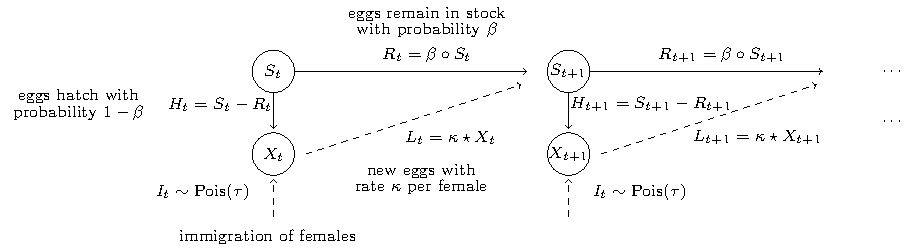
\includegraphics[scale=0.85]{figure/flowchart_ingarch_poisson.pdf}
\caption{Visualization of the Poisson INGARCH(1, 1) formulation \eqref{eq:R_t}--\eqref{eq:juv_t_v2} as a flow chart. Solid lines represent results of binomial thinning, dashed lines Poisson thinning or immigration. Note that the two solid arrows starting at $S_t$ do not represent independent binomial thinnings as by construction  $R_t + H_t = S_t$.}
\label{fig:ingarch_flowchart_poisson}
\end{figure}

\begin{enumerate}
\item $X_t$ is the number of females in the population at time $t$. Each of them stays alive for one time period and produces a $\text{Pois}(\kappa)$-distributed number of eggs with female offspring (eggs with male offspring are ignored). The total number of such eggs \textit{laid} at time $t$ is denoted by $L_t = \kappa \star X_t$.
\item Eggs laid at time $t$ enter into a \textit{stock} at time $t + 1$, with the number of eggs in stock at time $t + 1$ denoted by $\juv_{t + 1}$.
\item At each time $t$, each of the $S_t$ eggs in the stock can either remain there (with probability $\beta$) or hatch, thus being removed from the stock (with probability $1 - \beta$). The \textit{remaining} eggs $R_t = \beta \circ S_t$ form part of $S_{t + 1}$.
\item If an egg from $S_t$ \textit{hatches}, it releases a new female into $X_t$. The number of eggs hatching at time $t$ is denoted by $H_t = S_t - R_t$.
\item At each time $t$, a $\text{Pois}(\tau)$ distributed number $I_t$ of females \textit{immigrate} into the population.
\end{enumerate}
Note that a related model where the Poisson thinning in equation \eqref{eq:S_t_thinning_Poisson} is replaced by a binomial thinning has been introduced in \cite{Bracher2019}.

\subsection{The Poisson INGARCH($p$, $q$) model}
\label{subsec:poissonpq}

An extension of the thinning-based representation \eqref{eq:R_t}--\eqref{eq:juv_t_v2} to the INGARCH($p$, $q$) case is given by

\begin{align}
X_t & = I_t + H_t \label{eq:Xt_thinning_pq}\\
S_t & = \sum_{j = 1}^q R_{t - j, j} \ \ + \ \ \sum_{i = 1}^p L_{t - i, i}
\end{align}
where
\begin{align}
L_{t, i} & = \kappa_i \star X_t\\
(R_{t, 1}, \dots, R_{t, q}, H_t) \ \mid \ S_t & \sim \text{Mult}\left(S_t; \beta_1, \dots, \beta_q, 1 - \sum_{j = 1}^q \beta_j\right)\label{eq:R_t_mult}
\end{align}
and $\kappa_i, \beta_j > 0, \sum_{j = 1}^q \beta_j < 1$. For the initialization we fix $X_{-p + 1}, \dots, X_0$ and set $S_{u} \sim \text{Pois}(\eta_u)$ for $s = -q + 1, \dots, 0$. Again, the parameters $\beta_{1}, \dots, \beta_q$ are the same as in the original formulation \eqref{eq:lambda_t_pq}. The remaining parameters can be obtained as $\nu = \tau \times \left(1 - \sum_{j = 1}^q\beta_j \right)$ and $\alpha_i = \kappa_i \times \left(1 - \sum_{j = 1}^q\beta_j \right)$. For the initialization, one needs to set $\lambda_s = (1 - \sum_{j = 1}^q\beta_s) \times \eta_s, s = 1 - q, \dots, 0$.

In terms of the interpretation from the previous section the extension has the following implications. A visualization can be found in Figure \ref{fig:ingarch_flowchart_poisson_pq}.
\begin{itemize}
\item Eggs laid by females alive at $t$ cannot only enter into $S_{t + 1}$, but also $S_{t + 2}, \dots, S_{t + p}$. The number of such eggs entering into $S_{t + i}$ is $L_{t, i}$.
\item In the stock, eggs can ``skip'' time periods and move forward up to $q$ periods in one step. The number of eggs moving from $S_t$ directly to $S_{t + j}$ is denoted by $R_{t, j}$.
\end{itemize}
Formulation \eqref{eq:R_t_mult} implies $H_t + \sum_{j = 1}^q R_{t, j} = S_t,$ meaning that the $S_t$ eggs can take a variety of paths, but no egg is lost or added to the system as a whole in this step. Note that a similar construction is used in the INAR($p$) model as defined by Alzaid and Al-Osh \cite{Alzaid1990}.

\begin{figure}[h!]
\center
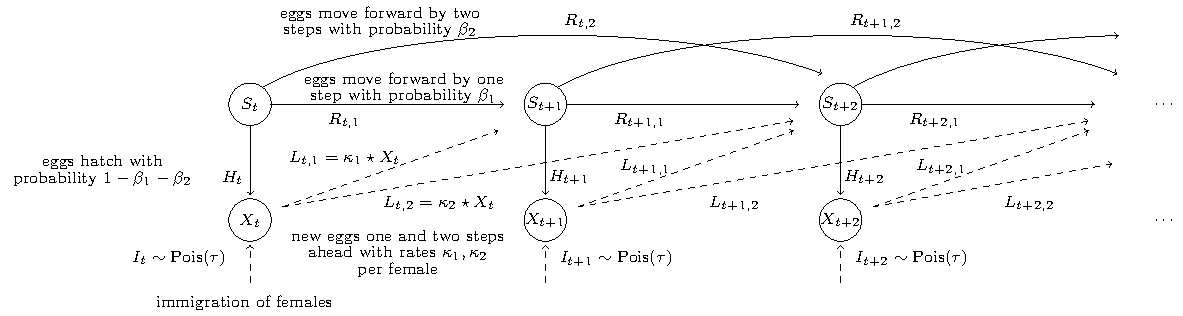
\includegraphics[scale = 0.8]{figure/flowchart_ingarch_poisson_pq.pdf}
\caption{Visualization of a Poisson INGARCH(2, 2) model as a flow chart. Solid lines represent results of multinomial thinning, dashed lines Poisson thinning. Note that the three solid arrows starting at $S_t$ do not represent independent thinnings as they are linked by the multinomial distribution and necessarily sum up to $S_t$.}
\label{fig:ingarch_flowchart_poisson_pq}

\end{figure}


\subsection{The compound Poisson INGARCH(1, 1) model}

A compound Poisson INGARCH(1, 1) process $\{X_t, t \in \mathbb{Z}\}$ equivalent to \eqref{eq:N_CP_original}--\eqref{eq:lambda_CP_original} is obtained by extending \eqref{eq:R_t}--\eqref{eq:juv_t_v2} to
\begin{align}
R_t & = \beta \circ S_t \label{eq:R_t_CP}\\
H_t & = S_t - R_t \label{eq:H_t_CP}\\
L_t & = \kappa \star X_t \label{eq:L_t_CP}\\
X_t & = \psi *_G (I_t + H_t)\label{eq:X_t_CP} \\
S_t & = R_{t - 1} + L_{t - 1}.\label{eq:juv_t_CP}
\end{align}
The employed operator $*_G$ is defined as
$$
\psi *_G N = \sum_{i = 1}^N Z_i \ \ \ \text{ with } \ \ \ Z_i \stackrel{\text{ind}}{\sim} G(\psi)
$$
and thus denotes summing over independent samples from a secondary distribution $G(\psi)$. The parameters $\beta$ and $\psi$ as well as the type of the secondary distribution $G$ are shared across the two formulations. The remaining parameters of the original formulation can be recovered as
$
\nu = \mu_\psi(1 - \beta)\tau$ and $ \ \
\alpha = \mu_\psi(1 - \beta)\kappa.
%; \ \
% \lambda_0 = \mu_\psi \left(\tau + \frac{1 - \beta}{\beta} \times \eta\right)
$
Concerning the initialization, equivalence is achieved by setting $\lambda_0 = \mu_\psi\times \left\{\tau + (1 - \beta)/\beta \times \eta\right\}$.

The interpretation provided in Section \ref{subsec:poisson11} can be adapted as follows, see also Figure \ref{fig:ingarch_flowchart}:
\begin{itemize}
\item Hatching eggs do not just release one new female, but a $G(\psi)$-distributed number.
\item Immigration consists of a $\text{Pois}(\psi)$-distributed number $I_t$ of hatching eggs, each of which releases a $G(\psi)$-distributed number of new females into the population.
\end{itemize}
The biological analogy is somewhat stretched here. It could be made more fitting by thinking of ``clusters'' or ``masses'' of eggs rather than single eggs, as e.g.\ in Neyman's \cite{Neyman1939} seminal work on compound count distributions. The extension to the compound Poisson setting translates directly to higher-order models as discussed in the previous section, but we omit details.

\begin{figure}[h!]
\center
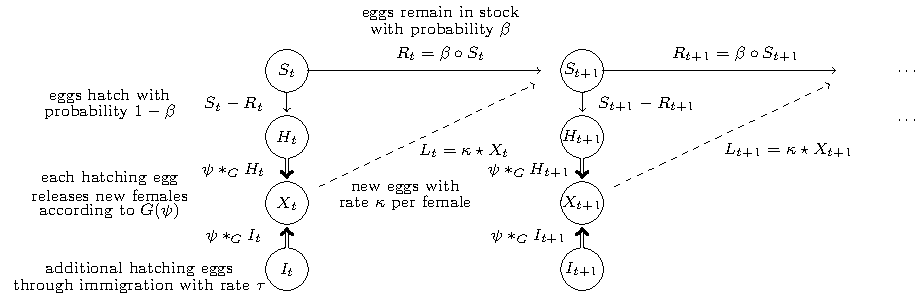
\includegraphics[scale = 0.8]{figure/flowchart_ingarch_cp.pdf}
\caption{Visualization of the CP-INGARCH(1, 1) formulation \eqref{eq:R_t}--\eqref{eq:juv_t_v2} as a flow chart. Solid lines represent results of binomial thinning, dashed lines Poisson thinning, double lines thinning with $*_G$. Note that the two solid arrows starting at $S_t$ do not represent independent binomial thinnings as by construction  $R_t + H_t = S_t$.}
\label{fig:ingarch_flowchart}
\end{figure}

% Thinning-based formulations of INGARCH(1, 1) models also appear in \cite{Ferland2006} and \cite{Goncalves2015}. However, these take the form of successive approximations approaching the INGARCH(1, 1) in the limit and thus provide a less direct handle on stochastic properties of the process. 


\section{Derivation of some stochastic properties}

We now discuss the derivation of some stochastic properties of the considered models via their reformulation. We focus on the CP-INGARCH(1, 1) model and exploit a link to branching process theory arising from the new representation.

\subsection{Geometric ergodicity}

Fokianos et al \cite{Fokianos2009} showed that a perturbed version of the Poisson INGARCH(1, 1) model is geometrically ergodic and Neumann \cite[Theorem 3.1]{Neumann2011} proved geometric ergodicity of a more general class of Poisson autoregressive models. Ergodicity of various other generalizations has been adressed by several authors \citep{Davis2016, Douc2013, Neumann2011}. Goncalves et al \citep{Goncalves2015} cover ergodicity (but not geometric ergodicity) of CP-INGARCH models. A proof of geometric ergodicity of the GP-INGARCH(1, 1) model along the lines of \cite{Neumann2011} has been sketched by Zhu \citep{Zhu2012}. Higher-order Poisson INGARCH models have been addressed more recently by Neumann \citep{Neumann2021}, while Doukhan et al \citep{Doukhan2021} treat a more general class not limited to conditional Poisson distributions. Mixing properties of non-stationary versions have been considered, too \cite{Doukhan2021a}. %  Other proofs of (geometric) ergodicity of INGARCH models have been given in the following works. Neumann \citep{Neumann2011} provides a contractive condition for ergodicity of a more general model class which includes non-linear autoregressive models, but also the Poisson INGARCH(1, 1). Zhu \citep{Zhu2012} states that the same technique can also be used to establish geomtric ergodicity of the GP-INGARCH(1, 1) model. Ergodicity of broader classes which are not limited to a conditional Poisson or generalized Poisson distribution have been considered by Douc et al \citep{Douc2013} and Davis and Liu \cite{Davis2016}. Goncalves et al \cite{Goncalves2015} established ergodicity (but not geometric ergodicity) of CP-INGARCH models. %, including higher-order models. % Multivariate Poisson INGARCH models have been analyzed by Fokianos et al \cite{Fokianos2020}.% However, to our best knowledge, geometric ergodicity has so far only been established for the Poisson INGARCH(1,1) model.\todo{Add Fokianos multivariate}

All of the mentioned arguments can be described as technically involved. As noted by Neumann \cite{Neumann2011}, the difficulty lies in the fact that the process $\{X_t\}$ is discrete-valued, while the conditional mean process $\{\lambda_t\}$ is real-valued. The re-formulation \eqref{eq:R_t_CP}--\eqref{eq:juv_t_CP} involves exclusively integer-valued processes, and allows us to exploit results from branching process theory. Substituting $X_{t - 1} = \psi *_G I_t + \psi *_G H_t$ (equation \eqref{eq:X_t_CP}) in \eqref{eq:juv_t_CP}, $\{\juv_t\}$ can be written as
\begin{align}
% \juv_t = \underbrace{R_{t - 1}}_{= \beta \circ S_{t - 1}} + \kappa \star \{\psi *_G (S_{t - 1} - R_{t - 1})\} + \kappa \star (\psi *_G I_{t - 1}). \label{eq:recursion_S}
\juv_t = \underbrace{R_{t - 1}}_{= \beta \circ S_{t - 1}} \ + \ \kappa \star (\psi *_G \underbrace{H_{t - 1}}_{ = S_{t - 1} - R_{t - 1}}) \ + \ \kappa \star (\psi *_G I_{t - 1}). \label{eq:recursion_S}
\end{align}
Here, $\kappa \star (\psi *_G I_{t - 1})$ represents eggs laid by females immigrated at $t - 1$. The term  $R_{t - 1}$ contains eggs remaining from $ \juv_{t - 1}$, while $\kappa \star (\psi *_G H_{t - 1})$ are new eggs laid by ``native'' females which themselves had hatched from the stock at time $t - 1$. Each egg from $S_{t - 1}$ thus contributes to $S_t$ in exactly one of two ways. Either it remains in the stock itself, entering $S_t$ via $R_{t - 1}$, which happens with probability $\beta$. Or, with probability $1 - \beta$, it enters into $H_{t - 1}$ and releases a $G(\psi)$-distributed number of new females into $X_{t - 1}$. These in turn each contribute new eggs to $S_t$ according to a $\text{Pois}(\kappa)$ distribution. Denoting the number of eggs contributed by the $i$-th of the $S_{t - 1}$ eggs from $t - 1$ by $A_{i, t - 1}$, we thus have
\begin{align}
A_{k, t - 1} & = \begin{cases}
1 & \text{with probability } \beta\\ % \ \ \ \ \ \ \  (\text{contribution via } R_{t - 1}) \\
\kappa \star (\psi *_G 1) & \text{with probability } 1 - \beta % \ \ (\text{ contribution via } \kappa \star (\psi *_G H_{t - 1})),
\label{eq:Z_t_i}
\end{cases}
% & \ \ \ \ \ \ \text{independently for each } i
\end{align}
independently for each $k$. Setting
\begin{align}
I^*_t & = \kappa\star (\psi *_G I_{t - 1}) \label{eq:I_star}
\end{align}
we can then re-write recursion \eqref{eq:recursion_S} as
$$
\juv_t = \sum_{k = 1}^{\juv_{t - 1}} A_{k, t - 1} \ \ + \ \ I^*_t.
$$
Thus, $\{\juv_t\}$ is a Galton-Watson branching process where the offspring distribution \eqref{eq:Z_t_i} is a specific one-inflated compound distribution. %, specifically, $A_{t, i}$ is a $G(\psi)$-stopped sum of Poisson random variables. 
The immigration distribution \eqref{eq:I_star} is defined by two compounding steps. % This follows from the fact that given $I_t$,  %are generated by two compounding steps. % and thus follow a Poisson Poisson compound or Neyman type A distribution with parameters $\kappa$ and $\tau$ \cite{Masse2005}.

Theory on branching processes with immigration, specifically Theorem 1 from Pakes \cite{Pakes1971} tells us that $\{\juv_t\}$ is geometrically ergodic if (a) $\mathbb{E}(A_{i, t}) < 1$, (b) $\mathbb{E}[(A_{i, t} + 1)\log(A_{i, t} + 1)] < \infty$, (c) $\mathbb{E}(I^*_t) < \infty$. These conditions are easily verified for $\{S_t\}$ provided that $\kappa\mu_\psi < 1$ and, as previously assumed, $\mu_I, \sigma^2_I, \sigma^2_\psi < \infty$.
%\begin{itemize}
%\item[(a)] $\mathbb{E}(A_{i, t}) < 1$,
%\item[(b)] $\mathbb{E}[(A_{i, t} + 1)\log(A_{i, t} + 1)] < \infty$,
%\item[(c)] $\mathbb{E}(I^*_t) < \infty$.
%\end{itemize}
% Condition (a) holds if $\kappa\mu_\psi < 1$. For condition (b) note that $\mathbb{E}[(A_{i, t} + 1)\log(A_{i, t} + 1)] < \mathbb{E}(A_{i, t}^2)$. As $A_{i, t}$ comes from a mixture of two distributions which both have finite second moments (noting that $\text{Var}[\kappa \star (\psi *_G 1)] = \kappa(\mu_\psi + \sigma^2_\psi) < \infty$ \todo{re-check!}) we have $\mathbb{E}(A_{i, t}^2) < \infty$. Condition (c) holds as $\mathbb{E}(I^*_t) = \kappa\mu_\psi\tau < \infty$.

% (For completeness we note that $\text{Var}[\kappa \star (\psi *_G 1)] = \mathbb{E}[\text{Var}\{\kappa \star (\psi *_G 1)\} \ \mid \ \psi *_G 1] + \text{Var}[\mathbb{E}\{\kappa \star (\psi *_G 1)\}  \ \mid \ \psi *_G 1] = \kappa\mu_\psi $)

As in Fokianos et al \cite{Fokianos2009}, Proposition 1 from Meitz and Saikkonen \cite{Meitz2008} can then be used to show that geometric ergodicity of $\{S_t\}$ is inherited by the joint process $\{(\juv_t, R_t, H_t, X_t, L_t)\}$. %, see Appendix \ref{appendix:proof_meitz}.
Even though it is in principle sufficient to initialize the process with $R_0$ and $X_0$ as in Section \ref{sec:alternative_formulation}, we now assume that $\{(\juv_t, R_t, H_t, X_t, L_t)\}$ is initialized by a vector $(s_0, r_0, h_0, x_0, l_0)$. Geometric ergodicity of the joint process is then established by verifying two conditions (Assumption 1 in \cite{Meitz2008}):

\begin{enumerate}
% \item Given $(\juv_u, R_u, H_u, X_u, L_u), u < t$ and $\juv_t$, $(R_t, H_t, X_t, L_t)$ depends only on $\juv_t$. This is straightforward to see from equations \eqref{eq:juv_t}--\eqref{eq:L_t} or Figure \ref{fig:ingarch_flowchart}.
\item Given $S_t$, $(R_t, H_t, X_t, L_t)$ is independent of all $\juv_u, R_u, H_u, X_u, L_u, u < t$. It is straightforward to see from equations \eqref{eq:R_t_CP}--\eqref{eq:juv_t_CP} or the graphical representation in Figure \ref{fig:ingarch_flowchart} that this is the case.
\item There is an $n \geq 1$ such that for all $t > n$, the generation mechanism of $\juv_t \ \mid \ \juv_0 = s_0, R_0 = r_0, H_0 = h_0, X_0 = x_0, L_0 = l_0$ has the same structure as that of $\juv_t \ \mid \ \juv_n = \tilde{s}_n$, where $\tilde{s}_n$ is some function of $(s_0, r_0, h_0, x_0, l_0)$. As $(s_0, r_0, h_0, x_0, l_0)$ only impacts the further course of the process $\{\juv_t\}$ through $\juv_1 = l_0 + r_0$, this is the case for $n = 1$. % and $\tilde{s}_1 = l_0 + r_0$.
\end{enumerate}
% This proves geometric ergodicity of the joint process $\{(\juv_t, R_t, X_t, L_t\}$ if $\kappa\mu_\psi < 1$ (and $\sigma_\psi^2 < \infty$, as assumed since Section \ref{sec:original_formulation}).

\subsection{Existence of higher moments}

Existence of higher-order moments of CP-INGARCH(1, 1) models with time-constant $\psi$ has been proven in \cite{Silva2016}, but the proof is quite involved. Representation \eqref{eq:R_t_CP}--\eqref{eq:juv_t_CP} allows again for a more condensed argument. It is known that if the offspring and immigration distributions of a subcritical Galton-Watson branching process have finite $r$-th moments, this is also the case for the limiting-stationary distribution \cite[Sec. 4]{Lange1981}. Both conditions are fulfilled for $\{S_t\}$ if the $r$-th moment of $G(\psi)$ is finite and $\kappa\mu_G < 1$:

\begin{itemize}
\item A randomly stopped sum $Y = \sum_{i = 1}^N Z_i$ of i.i.d. random variables $Z_i$ has finite $r$-th moments if $N$ and the $Z_i$ have finite $r$-th moments \cite[Theorem 5.2]{Gut2009}. The Poisson distribution has finite moments of any order. Thus, if the $r$-th moment of $G(\psi)$ is finite, this also holds for $\kappa \star (\psi *_G 1)$ and thus the offspring distribution from \eqref{eq:Z_t_i}.
\item Similar arguments imply that if $G(\psi)$ has a finite $r$-th moment, this is also the case for $\psi *_G I_{t - 1}$ and in a second step the immigration process $I^*_t = \kappa \star(\psi *_G I_{t - 1})$ from equation \eqref{eq:I_star}.
\end{itemize}
Consequently, the limiting-stationary distribution of $\{S_t\}$ has finite moments up to order $r$ if this is the case for the secondary distribution $G(\psi)$ (while $\kappa\mu_G < 1$). Similar arguments imply that finiteness of moments translates to $H_t = (1 - \beta) \circ S_t$, $\psi *_G H_t$ and ultimately $X_t = \psi *_G I_t + \psi *_G H_t$.
%
%\subsection{Consistency and asymptotic normality of moment estimators}
%
%Use same argument as in Weiss and Schweer 2016, exploiting Ibragimov 1962. Derive stationary mean, variance, acf for (1, 1) case, should be straightforward. Maybe even try getting the elements of the covariance matrix.

\subsection{Approximating the limiting-stationary distribution}

As $\{X_t\}$ is ergodic, the limits % \todo{Add example with computation times? Distinction of h-step ahead distributions and using matrix inverse; possibly check setting like $\alpha = 0.2, \beta = 0.75$.}
$$
p_i = \lim_{t \rightarrow \infty} \text{Pr}(X_t = i \ \mid R_0 = r_0, X_0 = x_0)
$$
exist and are independent of the initialization of the process (in the following we therefore suppress the condition on $r_0, x_0$ in the notation). However, even in the Poisson case no closed form for the $p_i$ is known. For INARCH(1) models, i.e. the special case $\beta = 0$ of the INGARCH(1, 1), a Markov chain approach can serve to approximate the $p_i$ with arbitrary precision \cite{Weiss2010}. This is based on the fact that the INARCH(1) is a discrete first-order Markov chain so that
$$
\text{Pr}(X_t = i) = \sum_{j = 0}^\infty p_{j|i} \times \text{Pr}(X_{t - 1} = j).
$$
Here, $p_{j|i} = \text{Pr}(X_t = i \ | \ X_{t - 1} = j) $ is the transition probability from $j$ to $i$. Choosing $T$ sufficiently large, the approximation is given by
$$
p_i \approx \text{Pr}(X_T = i),
$$
where $\text{Pr}(X_T = i)$ can in turn be approximated by recursively computing
$$
\text{Pr}(X_t = i) \approx \sum_{j = 0}^M p_{j|i} \times \text{Pr}(X_{t - 1} = j),
$$
with sufficiently large $M$ and some suitable initialization of $X_0$ (e.g. starting close to the stationary mean).

This method, however, is not directly applicable to the INGARCH(1, 1) model \eqref{eq:N_CP_original}--\eqref{eq:lambda_CP_original} as $\{X_t\}$ is not a first-order Markov chain. Application to the joint process $\{(X_T, \lambda_t)\}$, which is a first-order Markov chain, is not feasible as $\lambda_t$ has a continuous support. Formulation \eqref{eq:R_t}--\eqref{eq:juv_t_v2}, however, enables us to apply the approximation
$$
p^{(S)}_i \approx \text{Pr}(S_T = i) \ \ \text{and} \ \ \text{Pr}(S_t = i) \approx \sum_{j = 0}^M p^{(S)}_{j|i} \times \text{Pr}(S_{t - 1} = j)
$$
with large $T$ and $M$ to the discrete-valued Markov chain $\{S_t\}$. The computation of the transition probabilities $p_{j|i}$ is slightly tedious, but without conceptual difficulty. Subsequently one can compute an approximation of the limiting stationary distribution of $X_t$ as
$$
p_i = \sum_{k = 0}^M p_k^{(S)} \times \text{Pr}(X_t = i \ \mid \ S_t = k).
$$
% While it is somewhat tedious to compute the transition probabilities $p^{(S)}_{j|i}$ of $\{S_t\}$ as well as the probabilities $\text{Pr}(X_t = i \ \mid \ S_t = k)$ linking $\{S_t\}$ and $\{X_t\}$, this approach allows to evaluate the $p_t$ with arbitrary precision.


%% Existence of three derivatives of the log likelihood function is shown by Fokianos et al. Then Jensen and Rahbek's law of large numbers for geometrically ergodic processes implies normality of the maximum likelihood estimators.

% \section{Discussion}

% We have provided an alternative representation of the compound \todo{to be extended} Poisson INGARCH(1, 1) model and used it to obtain several properties of the process. Notably, the fact that the process is geometrically ergodic could be useful for studies of the behaviour of conditional maximum likelihood estimators along the lines of \cite{Fokianos2009} and \cite{Zhu2012}. % This question has not yet been addressed as existing studies are limited to conditional least squares (CLS) estimators \cite{Silva2016} and Poisson quasi-maximum likelihood estimators \cite{AhmadXXX}.

% Mention that CLS estimator is normal according to Cardoso da Silva. PQML is normal according to Ahmad and Francq.

%\section{Moment-based estimation}
%
%Limiting stationary properties: Set $\xi = \alpha + \beta$ and denoting the conditional dispersion index of $X_t \ \mid \ \lambda_t$ by
%$$
%\delta = \frac{\text{Var}(X_t \ \mid \ \lambda_t)}{\lambda_t} = \frac{\sigma^2_\psi + \mu_\psi^2}{\mu_\psi}.
%$$
%Then:
%$$
%\mu = \frac{\nu}{1 - \xi}, \ \ \sigma^2 = \frac{1 - \xi^2 + \alpha^2}{1 - \xi^2} \cdot \delta\mu, \ \ \rho(d) = \alpha\cdot \frac{1 - \beta\xi}{1 - \xi^2 + \alpha^2}\cdot \xi^{d - 1}
%$$
%
%Moment estimators:
%\begin{align*}
%\hat{\xi} & = \frac{\hat{\rho}(2)}{\hat{\rho}(1)}\\
%\hat{\nu} & = \hat{\mu}\cdot(1 - \hat{\xi})\\
%\hat{\alpha} & = \frac{(1 - \hat{\xi}^2) - \sqrt{(1 - \hat{\xi}^2) \cdot [1 - \hat{\xi}^2 - 4\hat\rho(1)\cdot\{\hat\rho(1) - \hat{\xi})\}]}}{2\{\hat\rho(1) - \hat{\xi}\}}\\
%\hat{\beta} & = \hat\xi - \hat\alpha\\
%\hat{\delta} & = \frac{\hat\sigma^2}{\hat\mu} \cdot \frac{1 - \hat\xi^2}{1 - \hat\xi^2 + \hat\alpha^2}
%\end{align*}
%
%
%For Poisson case one might derive the precise expressions.

% \newpage

\appendix
\section{Equivalence of the classical and thinning-based INGARCH formulations}
\label{appendix:proof}

\subsection{Poisson INGARCH(1, 1)}
\label{subsec:derivation_poisson11}

We demonstrate that the process $\{X_t, t \in \mathbb{N}_0\}$ from \eqref{eq:R_t}--\eqref{eq:juv_t_v2} is equivalent to the Poisson INGARCH(1, 1) process \eqref{eq:X_t_original}--\eqref{eq:lambda_t}. We start by decomposing $L_t, t \in \mathbb{N}_0$ and $S_0$ by when the respective eggs will hatch. We denote by $L_t^{(i)}$ the number of eggs laid at time $t$ and hatching at $t + i$ and by $S^{(i)}_0$ the number of eggs initially in the stock and hatching at time $i$ (note that $L_t^{(i)}$ is not to be confused with $L_{t, i}$ from Section \ref{subsec:poissonpq}). This implies
\begin{equation}
% L_t = \sum_{i = 1}^\infty L_t^{(i)}, \ \ \ 
% R_0 = \sum_{i = 1}^\infty R_0^{(i)}, \ \ \ 
H_t = \sum_{i = 1}^{t} L_{t - i}^{(i)} \ \ + \ \ S_0^{(t)}.
% R_t & = \sum_{i = 1}^t \sum_{j > i} L_{t - i}^{(j)} \ \ + \ \ \sum_{j > t} R_0^{(j)}.
\label{eq:sums}
\end{equation}
An egg laid at time $t$ has a probability of $\beta^{i - 1}(1 - \beta)$ to hatch at time $t + i, i = 1, 2, \dots$, and thus be part of $L_t^{(i)}$ (it has to remain in the stock $i - 1$ times and then hatch). The Poisson splitting property \cite{Kingman1993} then implies that given $X_t$, the $L_t^{(i)}$ are independently Poisson distributed,
$$
L_t^{(i)} \mid X_t \stackrel{\text{ind}}{\sim} \text{Pois}(\beta^{i - 1}[1 - \beta]\kappa X_t). % ; \ \ L_t^{(i)} \perp L_t^{(j)} \mid X_t, i \neq j.
$$
We note that given $X_t$, $L_t^{(i)}$ does not have any impact on the further course of the process $\{X_t\}$ until time $t + i$. Also, given $X_t$, $L_t^{(i)}$ is independent of the past of $\{X_t\}$. We can thus extend the condition in the above and write
$$
L_t^{(i)} \mid X_{t + i - 1}, \dots, X_0 \stackrel{\text{ind}}{\sim} \text{Pois}(\beta^{i - 1}[1 - \beta]\kappa X_t). % ; \ \ L_t^{(i)} \perp L_t^{(j)} \mid X_t, i \neq j
$$
Moreover, again because, given $X_t$, $L_t^{(i)}$ only impacts the further process from $t + i$ onwards, it is clear that $L_t^{(i)} \perp L_u^{(j)} \mid X_t, X_u$ for $t < u < t + i$.

Now consider %\todo{there seems to be a slight switch in what index $t$ represents}
\begin{align}
X_t & = I_t \ \ + \ \ \underbrace{\sum_{i = 1}^{t} L_{t - i}^{(i)} \ \ + \ \ S_0^{(t)}}_{= H_t}, \label{eq:introduce_N_T}
\end{align}
where we substituted $H_t$ in equation \eqref{eq:X_t_v2} using equation \eqref{eq:sums}. In analogy to the above argument, $S_0^{(t)}$ is Poisson distributed with rate $\eta\beta^{t}(1 - \beta)$ and independent of all $X_u$ and $L_u^{(i)}, u \leq t - 1$. Conditioned on $X_{t - 1}, \dots, X_0$, we thus have that the term $X_t$ is a sum of independent Poisson random variables (as $I_t \sim \text{Pois}(\tau)$). This implies
$$
X_t \mid X_{t - 1}, \dots, X_0, \eta \sim \text{Pois}(\lambda_t)
$$
where the conditional expectation is given by
\begin{align*}
& \lambda_t = \mathbb{E}(I_t) \ \ + \ \ \sum_{i = 1}^t \mathbb{E}(L_{t - i}^{(i)} \ \mid \ X_{t- 1}, \dots, X_0) \ \ + \ \ \mathbb{E}(S_0^{(t)})\\
& \ \ \ = \ \ \tau \ \ \ \ \ + \ \ \sum_{i = 1}^t \beta^{i - 1}(1 - \beta)\kappa X_{t - i} \ \ \ \ \ \ \ \ \ \ + \ \ \beta^{t}(1 - \beta)\eta\\
\end{align*}
We can then re-write $\lambda_t$ as
\begin{align*}
\lambda_t & = (1 - \beta)\tau + (1 - \beta)\kappa X_{t - 1} + \beta \left\{\tau +    \sum_{i = 2}^t \beta^{i - 1}(1 - \beta)\kappa X_{t - i}  \ \ + \ \ \beta^{t - 1}(1 - \beta)\eta\right\}\\
& = \underbrace{(1 - \beta)\tau}_{\nu} \ + \ \underbrace{(1 - \beta)\kappa}_{\alpha} X_{t - 1} \ + \ \beta \lambda_{t - 1}
\end{align*}
for $t \geq 2$. This is the form a Poisson INGARCH(1, 1) model. We conclude by considering the initialization of the process, where we have
\begin{align*}
\lambda_1 = \mathbb{E}(X_1 \ \mid \ X_0) & = \tau + (1 - \beta)\kappa X_0 + \beta(1 - \beta)\eta\\
& =  \tau (1 - \beta) + (1 - \beta)\kappa X_0 + \beta  \left\{\tau + (1 - \beta) \times \eta \right\},
\end{align*}
meaning that we have to set $\lambda_0 =\tau + (1 - \beta)/\beta \times \eta$.

%\subsection{V2}
%
%We demonstrate that the process $\{X_t, t \in \mathbb{N}_0\}$ from \eqref{eq:R_t}--\eqref{eq:juv_t_v2} is equivalent to the Poisson INGARCH(1, 1) process \eqref{eq:X_t_original}--\eqref{eq:lambda_t}. We start by decomposing $L_t, t \in \mathbb{N}_0$ and $R_0$ by when the respective eggs will hatch. We denote by $L_t^{(i)}$ the number of eggs laid at time $t$ and hatching at $t + i$ and by $R^{(i)}_0$ the number of eggs initially in the stock and hatching at time $i$ (note that these are not to be confused with $L_{t, i}$ and $R_{o, i}$ from Section \ref{subsec:poissonpq}). This implies
%\begin{equation}
%% L_t = \sum_{i = 1}^\infty L_t^{(i)}, \ \ \ 
%% R_0 = \sum_{i = 1}^\infty R_0^{(i)}, \ \ \ 
%H_t = \sum_{i = 1}^{t} L_{t - i}^{(i)} \ \ + \ \ R_0^{(t)}.
%% R_t & = \sum_{i = 1}^t \sum_{j > i} L_{t - i}^{(j)} \ \ + \ \ \sum_{j > t} R_0^{(j)}.
%\label{eq:sums}
%\end{equation}
%Denote the probability that an egg laid at time $t$ hatches at time $t + i, i = 1, 2, \dots$, thus becoming part of $L_t^{(i)}$, by $p_i$; it is easy to show that $p_i = \beta^i(1 - \beta)$. The Poisson splitting property \cite{Kingman1993} then implies that given $X_t$, the $L_t^{(i)}$ are independently Poisson distributed,
%$$
%L_t^{(i)} \mid X_t \stackrel{\text{ind}}{\sim} \text{Pois}(p_i\kappa X_t). % ; \ \ L_t^{(i)} \perp L_t^{(j)} \mid X_t, i \neq j.
%$$
%We note that given $X_t$, $L_t^{(i)}$ does not have any impact on the further course of the process $\{X_t\}$ until time $t + i$. Also, given $X_t$, $L_t^{(i)}$ is independent of the past of $\{X_t\}$. We can thus extend the condition in the above and write
%$$
%L_t^{(i)} \mid X_{t + i - 1}, \dots, X_0 \stackrel{\text{ind}}{\sim} \text{Pois}(p_i\kappa X_t). % ; \ \ L_t^{(i)} \perp L_t^{(j)} \mid X_t, i \neq j
%$$
%Moreover, again because, given $X_t$, $L_t^{(i)}$ only impacts the further process from $t + i$ onwards, it is clear that $L_t^{(i)} \perp L_u^{(j)} \mid X_t, X_u$ for $t < u < t + i$.
%
%Now consider %\todo{there seems to be a slight switch in what index $t$ represents}
%\begin{align}
%X_t & = I_t \ \ + \ \ \underbrace{\sum_{i = 1}^{t} L_{t - i}^{(i)} \ \ + \ \ R_0^{(t)}}_{= H_t}, \label{eq:introduce_N_T}
%\end{align}
%where we substituted $H_t$ in equation \eqref{eq:X_t_v2} using equation \eqref{eq:sums}. In analogy to the above argument, $R_0^{(t)}$ is Poisson distributed with rate $p_t\eta$ and independent of all $X_u$ and $L_u^{(i)}, u \leq t - 1$. Conditioned on $X_{t - 1}, \dots, X_0, \eta$, we thus have that the term $X_t$ is a sum of independent Poisson random variables (as $I_t \sim \text{Pois}(\tau)$). This implies
%$$
%X_t \mid X_{t - 1}, \dots, X_0, \eta \sim \text{Pois}(\lambda_t)
%$$
%with some $\lambda_t$, which we will determine in the next step. To this end, denote by $\xi_{t} = \mathbb{E}(S_t  \ \mid \ X_{t - 1}, \dots, X_0)$. We note that for $t = 2, 3, \dots$
%\begin{align}
%\lambda_t & = (1 - \beta)\xi_t + \tau
%\label{eq:EXt}\\
%\xi_t & = \beta \times \xi_{t - 1} + \kappa X_t.
%\label{eq:ESt}
%\end{align}
%The latter recursion is a direct consequence of the fact that $p_{i + 1} = \beta p_i$ and thus $\mathbb{E}(L^{(i + 1)}_t \ \mid \ X_t) = \beta\mathbb{E}(L^{(i)}_t \ \mid \ X_t)$ and $\mathbb{E}(R^{(t + 1)}_0) = \beta\mathbb{E}(R^{(t)}_0)$. Plugging \eqref{eq:EXt} into \eqref{eq:ESt} we then obtain
%$$
%\frac{\lambda_t - \tau}{1 - \beta} = \beta \times \frac{\lambda_{t - 1} - \tau}{1 - \beta} + \kappa X_{t - 1}
%$$
%which simplifies to
%$$
%\lambda_t = \underbrace{(1 - \beta)\tau}_{\nu} \ + \ \underbrace{(1 - \beta)\kappa}_{\alpha} X_{t - 1} \ + \ \beta \lambda_{t - 1}.
%$$
%This is the form a Poisson INGARCH(1, 1) model. We conclude by considering the initialization of the process, where we have
%\begin{align*}
%\lambda_1 = \mathbb{E}(X_1 \ \mid \ X_0) & = \tau + (1 - \beta)\kappa X_0 + (1 - \beta)\eta\\ % \lambda_1 = \tau(1 - \beta) + (1 - \beta)\kappa X_0 + \beta\left(\tau + \frac{1 - \beta}{\beta} \times \eta \right),\\
%& =  \tau (1 - \beta) + (1 - \beta)\kappa X_0 + \beta  \left(\tau + \frac{1 - \beta}{\beta} \times \eta \right),
%\end{align*}
%meaning that we have to set $\lambda_0 =\tau + (1 - \beta)/\beta \times \eta$.
%
%\subsection{Poisson INGARCH($p, q$)}
%
%We now denote by
%$$
%L_t = \sum_{i = 1}^p L_{t, i}
%$$
%the total number of eggs laid at time $t$ (summed over the different entry times into $\{S_t\}$). This quantity can also be decomposed by when the eggs hatch. Denote as in the prevous section by $L_t^{(i)}$ the number of eggs laid at $t$ and hatching at $t + i$. We now decompose these even further and denote by $L_t^{(i, j)}, i \geq 1, j = 1, \dots, q$ the number of eggs laid at $t$, hatching at $t + i$ and having moved into $S_{t + i}$ directly from $S_{t + i - j}$ (i.e., having been part of $R_{t + i - j}^{(j)}$ in equation \eqref{eq:R_t_mult}; see interpretation in Section \ref{subsec:poissonpq}). We thus have the rather fine decomposition
%$$
%L_t = \sum_{i = 1}^\infty L_t^{(i)} = \sum_{i = 1}^\infty \sum_{j = 1}^q L_t^{(i, j)}
%$$
%
%The same decomposition is defined for the eggs entering the stock at initialization. We denote by $S_u^{(i)}, u = -q + 1, \dots, 0$ the number of eggs entering the process via $S_u$, hatching at $u + i$; and by $S_u^{(i, j)}, u = -q + 1, \dots, 0$ the number of eggs entering the process via $S_u$, hatching at $u + i$ and having been passed to $S_{u + i}$ from $S_{u + i - j}$ via $R_{u + i - j, j}$.
%
%This allows us to write
%\begin{align}
%H_t & = \sum_{i = 1}^{t + q - 1} L^{(i)}_{t - i} \ \ + \ \ \sum_{j = -q + 1}^{0} S_{j}^{(t - j)} \nonumber\\
%& = \sum_{i = 1}^{t + q - 1} \sum_{k = 1}^q L^{(i, k)}_{t - i} \ \ + \ \ \sum_{j = -q + 1}^{0} \sum_{k = 1}^q S_{j}^{(t - j, k)}.\label{eq:Htpq}
%\end{align}
%
%Paralleling the arguments form the previous section it can be shown that given $X_{t - 1}, \dots, X_{-q + 1}$ all summands in \eqref{eq:Htpq} are independent Poisson random varianbles. This implies that $H_t$ and thus also $X_t = I_t + H_t$ are conditionally Poisson with a rate $\lambda_t$, which we will address in the next step.
%
%As in the previous section we consider the conditional expectation of $S_t$,
%$$
%\xi_t = \mathbb{E}(S_t \ \mid \ X_{t - 1}, \dots, X_{1 - p}),
%$$
%and note that
%$$
%\lambda_t = \left(1 - \sum_{j = 1}^q \beta_j \right) \times \xi_t.
%$$
%It is straightforward to see that
%$$
%\mathbb{E}(L_t^{i, j})
%$$
%
%  
%\begin{equation}
%\lambda_t = (1 - \beta)\xi_t + \tau
%\end{equation}
%and
%\begin{equation}
%\xi_t = \sum_{i = 1}^p \kappa_i X_{t - i} + \sum_{j = 1}^p \beta_i\xi_{t - j}
%\end{equation},
%which after some algebra leads to

% \newpage

\subsection{Poisson INGARCH($p, q$)}
\label{subsec:derivation_poissonpq}

The proof follows essentially the same steps as in Section \ref{subsec:poisson11}, but is somewhat lengthy due to the more complex recursive relationships. It has therefore been moved to the Supplementary Material.


\subsection{Compound Poisson INGARCH(1, 1)}

Setting $N_t = I_T + H_t$, the same arguments as in \eqref{subsec:derivation_poisson11} can be used to show that
$$
N_t \mid X_{t - 1}, \dots, X_0, \eta \sim \text{Pois}(\lambda_t/\mu_\psi)
$$
where the conditional expectation is given by
\begin{align*}
& \lambda_t/\mu_\psi = \mathbb{E}(I_t) \ \ + \ \ \sum_{i = 1}^t \mathbb{E}(L_{t - i}^{(i)}) \ \ + \ \ \mathbb{E}(R_0^{(t)})\\
& \ \ \ \ \ \ \ \ = \tau \ \ + \ \ \sum_{i = 1}^t \beta^{i - 1}(1 - \beta)\kappa X_{t - i} \ \ + \ \ \beta^{t - 1}(1 - \beta)\eta\\
\Leftrightarrow \ \ & \lambda_t = \mu_\psi \tau \ \ + \ \ \mu_\psi \times \sum_{i = 1}^t \beta^{i - 1}(1 - \beta)\kappa X_{t - i} \ \ + \ \ \mu_\psi\beta^{t - 1}(1 - \beta)\eta
\end{align*}
We can then re-write $\lambda_t$ as
\begin{align*}
\lambda_t & = \mu_\psi(1 - \beta)\tau + \mu_\psi(1 - \beta)\kappa X_{t - 1} + \beta \left[\mu_\psi\tau +   \mu_\psi \sum_{i = 2}^t \beta^{i - 1}(1 - \beta)\kappa X_{t - i}  \ \ + \ \ \mu_\psi\beta^{t - 2}(1 - \beta)\eta\right]\\
& = \underbrace{\mu_\psi(1 - \beta)\tau}_{\nu} \ + \ \underbrace{\mu_\psi(1 - \beta)\kappa}_{\alpha} X_{t - 1} \ + \ \beta \lambda_{t - 1}
\end{align*}
for $t \geq 2$. Combined with the relationship $X_t = \psi *_G N_t$ from equation \eqref{eq:introduce_N_T} this is the form a CP-INGARCH(1, 1) model as introduced in \eqref{eq:N_CP_original}--\eqref{eq:lambda_CP_original}. Concerning the initialization of the process, the same argument as in Section \ref{subsec:poisson11} implies that we have to set $\lambda_0 = \mu_\psi\times \left\{\tau + (1 - \beta)/\beta \times \eta\right\}$.



% \section*{References}

\bibliographystyle{plain}
\bibliography{bib_ingarch.bib}

\newpage

\section{Demonstration of equivalence for the INGARCH($p, q$) model}

We use an argument similar to the one from Section \ref{subsec:derivation_poisson11} to demonstrate that the classical formulation \eqref{eq:X_t_original}, \eqref{eq:lambda_t_pq} of the INGARCH($p, q$) model and the thinning-based version \eqref{eq:Xt_thinning_pq}--\eqref{eq:R_t_mult} are equivalent. Again we denote by $L_t^{(i)}$ the number of eggs laid by females from time $t$ and hatching at $t + i$. Extending on the notation from the previous section, we denote by $S^{(i)}_u, u = 1 - q, \dots, 0$ the number of eggs entering the stock via the initialization at time $u$ and hatching at time $u + i$. Generalizing equation \eqref{eq:introduce_N_T} we then have
$$
X_t = I_t \ \ + \ \ \underbrace{\sum_{i = 1}^{t + p - 1} L_{t - i}^{(i)} \ \ + \ \ \sum_{m = 1 - q}^0 S_m^{(t - m)}}_{= H_t}, \label{eq:introduce_N_T}
$$
for $t = 1, 2, \dots$. Arguments identical to those from the previous section imply that given $X_{t - 1}, \dots, X_{1 - p}$ all summands in the above equation are independently Poisson distributed, so that $X_t$, too, is conditionally Poisson with a rate $\lambda_t$.

The conditional expectation of $L_t^{(i)}$ is given by
\begin{equation}
\mathbb{E}(L_t^{(i)} \ \mid \ X_{t + i - 1}, \dots, X_{1 - p}) = \left(1 - \sum_{l = 1}^q \beta_l \right) \times \left(\sum_{k = 1}^p\ \kappa_k \pi_{i - k}\right) X_t,\label{eq:ELt}
\end{equation}
where we denote by $\pi_k$ the probability that an egg entering the stock at time $t$ is also in the stock at time $t + k$. The reasoning behind this relationship is that the $X_t$ females from time $t$ generate eggs entering at times $t + 1, \dots, t + p$ with rates $\kappa_1, \dots, \kappa_p$; these then have to also be present in the stock exactly $i - 1, \dots, i - p$ time points later, respectively, and then leave the stock (which happens with probability $1 - \sum_{l = 1}^q \beta_l$).

For the $\pi_i$, the recursion
\begin{align}
\pi_i = \sum_{j = 1}^q \beta_j \pi_{i - j}, \label{eq:recursion_pi}
\end{align}
with $\pi_0 = 1$ and $\pi_j = 0$ for $j < 0$ holds. This is because an egg which entered the stock at time $t$ can arrive in $S_{t + i}, i \geq 1$ from any of $S_{t + i - 1}, \dots S_{t + i - q}$ (even though some of these moves may not be possible if $i < q$; this will be reflected in $\pi_{i - j} = 0$). To do so, it needs to have arrived at the respective $S_{t + i - j}$ (which it does with probability $\pi_{i - j}$) and then make a $j$-step jump into $S_{t + i}$ (this happens with probability $\beta_j$).

We can now consider
\begin{align}
\lambda_t = \mathbb{E}(X_t \ \mid \ X_{t - 1}, \dots, X_{1 - p}) = & \ \tau 
\ + \ \sum_{i = 1}^{t + p - 1}\mathbb{E}(L^{(i)}_{t - i} \ \mid \ X_{t - 1}, \dots, X_{1 - p})
\ + \sum_{m = 1 - q}^0 \mathbb{E}(S_{m}^{(t + m)}  \ \mid \ X_{t - 1}, \dots, X_{1 - p}).\label{eq:lambda_t_pq_recursion1}
\end{align}

Focusing on the second summand and plugging in equation \eqref{eq:ELt}, we obtain
\begin{align*}
\sum_{i = 1}^{t + p - 1}\mathbb{E}(L^{(i)}_t \ \mid \ X_{t - 1}, \dots, X_{1 - p}) = & \left(1 - \sum_{l = 1}^q \beta_l\right) \times \left( \sum_{i = 1}^{t + p - 1} \sum_{k = 1}^p \kappa_k \pi_{i - k} X_{t - i}\right)\\
= & \left(1 - \sum_{l = 1}^q \beta_l\right) \times \left(\sum_{k = 1}^p \sum_{i = k}^{t + p - 1} \kappa_k \pi_{i - k} X_{t - i}\right).
\end{align*}
Note that in the last step we can start the last sum from $i = k$ rather than $i = 1$ as $\pi_{i - k} = 0$ for $i < k$. We can then further decompose this sum into
\begin{align}
= & \left(1 - \sum_{l = 1}^q \beta_l\right) \times \left(\underbrace{\sum_{k = 1}^p \kappa_k \pi_0 X_{t - k}}_{\text{corresponds to } i = k; \text{ note: } \pi_0 = 1} \ + \ \sum_{k = 1}^p \sum_{i = k + 1}^{t + p - 1} \kappa_k \pi_{i - k} X_{t - i}\right)\nonumber\\
= & \left(1 - \sum_{l = 1}^q \beta_l\right) \times \left\{\sum_{k = 1}^p \kappa_k X_{t - k} \ + \ \sum_{k = 1}^p \sum_{i = k + 1}^{t + p - 1} \kappa_k \times \underbrace{\left(\sum_{j = 1}^q \beta_j \pi_{i - k - j}\right)}_{\text{using equation \eqref{eq:recursion_pi}}} \times X_{t - i}\right\}\nonumber\\
= & \left(1 - \sum_{l = 1}^q \beta_l\right) \times \left\{\sum_{k = 1}^p \kappa_k X_{t - k} \ + \ \sum_{j = 1}^q \beta_j \times \left(\sum_{k = 1}^p \sum_{i = k + 1}^{t + p - 1} \kappa_k \times \pi_{i - k - j} \times X_{t - i}\right)\right\}\nonumber\\
= & \left(1 - \sum_{l = 1}^q \beta_l\right) \times \left\{\sum_{k = 1}^p \kappa_k X_{t - k} \ + \ \sum_{j = 1}^q \beta_j \times \left(\sum_{k = 1}^p \sum_{i = k + 1 - j}^{(t - j) + p - 1} \kappa_k \times \pi_{i - k} \times X_{(t - j) - i}\right)\right\}\nonumber\\
= & \left(1 - \sum_{l = 1}^q \beta_l\right) \times \left\{\sum_{k = 1}^p \kappa_k X_{t - k} \ + \ \sum_{j = 1}^q \beta_j \times \left(\sum_{k = 1}^p \sum_{i = 1}^{(t - j) + p - 1} \kappa_k \times \pi_{i - k} \times X_{(t - j) - i}\right)\right\}\label{eq:substitution_ELt}
\end{align}
where in the last step we can let the last sum start at $i = 1$ rather than $i = k + 1 - j$ as $\pi_{i - k} = 0$ for $i = 1, \dots, k - j$.

For the third term from equation \eqref{eq:lambda_t_pq_recursion1} we pursue a similar argument:

\begin{align}
\sum_{m = 1 - q}^0 \mathbb{E}(S_{m}^{(t + m)}  \ \mid \ X_{t - 1}, \dots, X_{1 - p}) & = \left(1 - \sum_{l = 1}^q \beta_l\right) \times \sum_{m = 1 - q}^0 \pi_{t - m}\rho_m\nonumber\\
& = \left(1 - \sum_{l = 1}^q \beta_l\right) \times \sum_{m = 1 - q}^0 \sum_{j = 1}^q \beta_j \pi_{t - j - k}\rho_m\nonumber\\
& =  \left(1 - \sum_{l = 1}^q \beta_l\right) \times\sum_{j = 1}^q \beta_j \times \left(\sum_{m = 1 - q}^0 \pi_{(t - j) - m}\rho_m\right).\label{eq:substitution_ESt}
\end{align}

Plugging the terms from \eqref{eq:substitution_ELt} and \eqref{eq:substitution_ESt} into \eqref{eq:lambda_t_pq_recursion1} we then get

\begin{align*}
\lambda_t = & \ \ \tau \ + \ \left(1 - \sum_{l = 1}^q \beta_l\right) \times \Bigg\{\sum_{k = 1}^p \kappa_k X_{t - k} \ + \ \sum_{j = 1}^q \beta_j \times \left(\sum_{k = 1}^p \sum_{i = 1}^{(t - j) + p - 1} \kappa_k \times \pi_{i - k} \times X_{(t - j) - i}\right) \\
& \ \ \ \ \ \ \ \ \ \ \ \ \ \ \ \ \ \ \ \ \ \  \ \ \ \ \ \ \ \ \ \ \ + \ \sum_{j = 1}^q \beta_j \times \left(\sum_{m = 1 - q}^0 \pi_{(t - j) - m}\rho_m\right)\Bigg\}.
\end{align*}

This can be re-ordered to
\begin{align*}
\lambda_t & = \left(1 - \sum_{l = 1}^q \beta_l\right) \times \tau \ + \ \left(1 - \sum_{l = 1}^q \beta_l\right) \times \left(\sum_{k = 1}^p \kappa_k X_{t - k}\right)\\
& \ \ \ + \sum_{j = 1}^q \beta_j \underbrace{\left(\tau \ + \  \sum_{k = 1}^p \sum_{i = 1}^{(t - j) + p - 1} \kappa_k \times \pi_{i - k} \times X_{(t - j) - i} \ + \ \sum_{m = 1 - q}^0 \pi_{(t - j) - m}\rho_m \right)}_{= \lambda_{t - j}}\\
& = \nu \ \ + \ \ \sum_{k = 1}^p \alpha_k X_{t - k} \ \ + \ \ \sum_{j = 1}^q \beta_j \lambda_{t - j},
\end{align*}
where
$$
\nu = \left(1 - \sum_{l = 1}^q \beta_l\right) \times \tau, \ \ \ \alpha_k = \left(1 - \sum_{l = 1}^q \beta_l\right) \times \kappa_k, k = 1, \dots, p.
$$
This is the form of a Poisson INGARCH($p, q$) model as defined in equation \eqref{eq:lambda_t_pq}.

Concerning the initialization, it can be shown that one needs to set $\lambda_s = (1 - \sum_{j = 1}^q\beta_s) \times \eta_s, s = 1 - q, \dots, 0$. This can be done using essentially the same argument as in the previous section, but we omit the somewhat lengthy details.


\end{document}